\chapter{Beyond Margins: Winner and Runner-up votes}
\label{chap6}

Building on our exploration of the Random Voting Model in the previous chapter, we now extend our investigation to other key electoral statistics and their relationship with voter turnouts. While we established that the RVM successfully predicts the universal specific margin distribution and connects turnout distributions to margin distributions across different electoral contexts, a natural question arises: Can the distribution of other relevant electoral statistics be uncovered using voter turnout distributions?

To address this question effectively, we require large datasets covering a range of different electoral scales. India, the world's largest democracy, regularly conducts elections involving vast electorates (960 million in 2024), and its publicly available election data spans multiple decades and electoral scales. The diversity of India's linguistic and cultural landscape further adds to the complexities of its electoral outcomes, making it an excellent testing ground for assessing the robustness of the RVM framework.

In this chapter, using empirical data from Indian elections spanning several decades and vastly different electoral scales, we demonstrate a strong correlation between the distributions of votes received by winners and runner-ups and voter turnouts. Leveraging this correlation and the RVM, we analytically predict the scaled distributions of the votes secured by winners and runner-ups using the corresponding turnout distributions. This prediction remarkably holds good at all the electoral scales -- from large parliamentary constituencies ($ \sim 10^6$ voters) down to the smallest polling booth levels ($\sim 10^2-10^3$ voters). Further, we show a rather surprising scale invariance of the margin distributions, a characteristic typical of Indian elections. 

\section{The Effective Number of Candidates}
While our previous analysis employed a fixed number of candidates ($n^c = 3$) for the Random Voting Model, here we refine our approach by introducing the concept of the effective number of candidates \cite{laakso1979effective}. This metric, widely used in political science, captures the actual level of competition more accurately than the raw count of candidates on a ballot.

The effective number of candidates is defined as:
\begin{equation}
    ^{(E)}n^c_i = \frac{1}{\sum_{k=1}^{n^c_i} (V_{ik} / T_{i})^2}.
    \label{eq:effc}
\end{equation}
In large electoral exercises such as those in India, even though many candidates join the fray, a few corner most of the votes. For instance, if all the votes are garnered by just one candidate, then $V_{i1}=T_i$, and $V_{ij}=0$ for $j=2, \dots n^c$. In this case, $^{(E)}n^c_i=1$. However, if all the votes are split equally among two candidates, $^{(E)}n^c_i=2$, thus, Eq. \ref{eq:effc} captures the idea of an effective number of candidates in $i$-th electoral unit.

By averaging over all the electoral units, we obtain:
\begin{equation}
    ^{(E)}\Tilde{n}^c =  \left[\frac{1}{N}\sum_{k=1}^{N}{}^{(E)}n^{c}_k \right],
\end{equation}
where $\left[\:*\:\right]$ denotes the operation of extracting the closest integer value. And $^{(E)}\Tilde{n}^c $ indicates the effective number of candidates for an entire election at different electoral scales.

From empirical data of Indian elections at different scales, we find $^{(E)}\Tilde{n}^c = 2$ at the polling booth (PB) level for the General Elections. However, for all the other three cases of Assembly Constituency in General Elections (AC-GE), Parliamentary Constituency in General Elections (PC-GE), and Assembly Constituency in State Elections (AC-SE), we obtain $^{(E)}\Tilde{n}^c = 3$. This insight allows us to adapt our modeling approach to better match the electoral reality at each scale.
\section{Relationship Between Turnout and Vote Distributions}
Depending on the electoral level considered, the winner and runner-up vote distributions have vastly different scales, with the winner vote distribution having wider support than the runner-up. However, when both distributions are scaled by their respective mean values (mean taken over all elections for which data is available), the winner and runner-up vote distributions -- $Q_{\widetilde{V_w}}(\widetilde{V_w})$ and $Q_{\widetilde{V_r}}(\widetilde{V_r})$ -- explicitly display a strong correlation with the corresponding scaled turnout distributions $Q_{\widetilde{T}}(\widetilde{T})$. Figure \ref{fig:turnout_winner_runnerup} shows this correlation for four different electoral scales in India.
\begin{figure}[H]
    \centering
    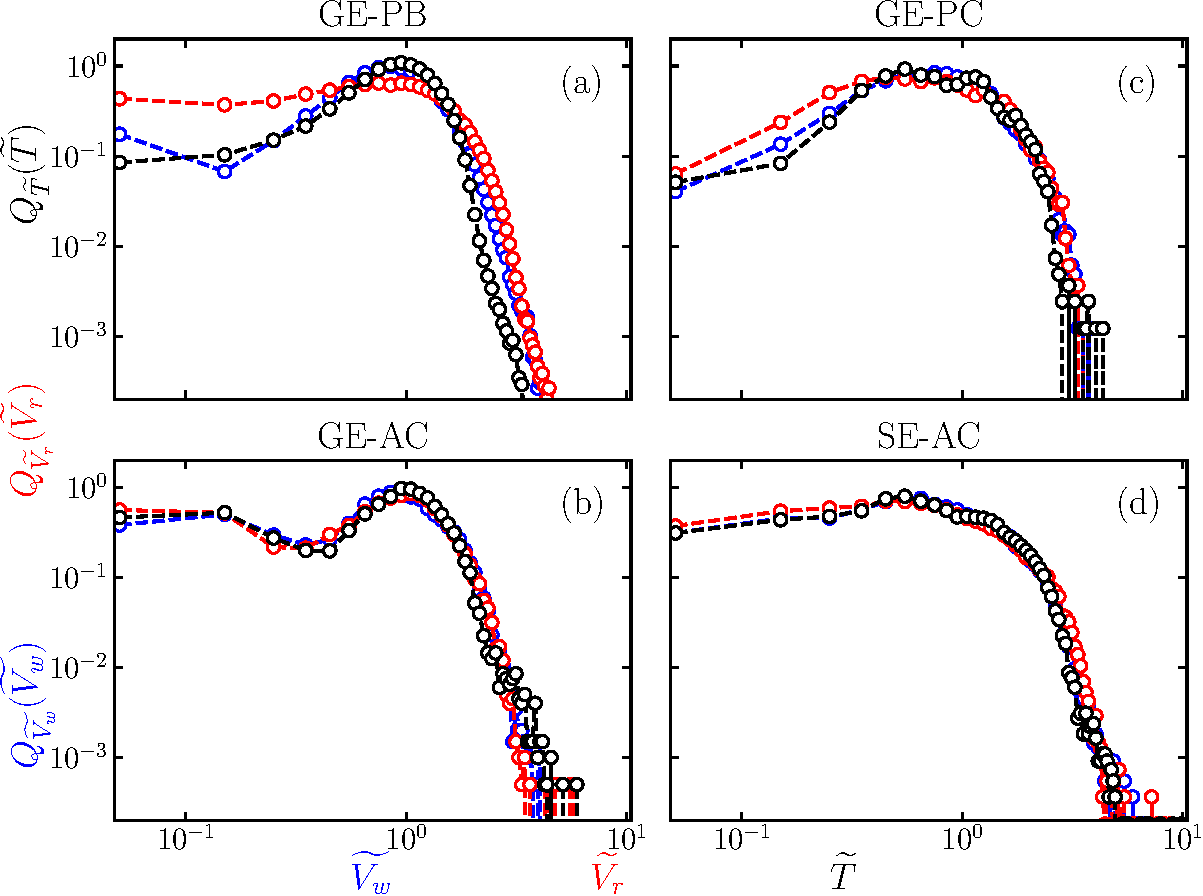
\includegraphics[width=\columnwidth]{chapters/chapter6/turnout_winner_runerup.pdf}
    \caption{Winner, runner-up vote distributions, and turnout distributions, scaled by their respective means. Notably, at larger electoral scales (AC / PC), the winner and runner-up distributions mimic the corresponding turnout distribution.}
    \label{fig:turnout_winner_runnerup}
\end{figure}
Remarkably, at larger electoral scales (Parliamentary and Assembly constituencies), not only the tail but the entire scaled distributions of winner and runner-up votes mimic the corresponding scaled turnout distribution (panel (b) and (c) and (d) in Fig. \ref{fig:turnout_winner_runnerup}). This strong correlation indicates that the turnout distribution contains crucial information about different election statistics and can be leveraged to predict the scaled vote distributions of the winner and the runner-up. To explore this possibility, we apply the Random Voting Model, which has already demonstrated effectiveness at predicting the scaled distribution of margins of victory.

\section{Predicting Vote Distributions from Turnout Distributions}
We now extend our analytical framework to derive the distributions of votes received by winners and runner-ups in the RVM.

\subsection{Random Voting Model: a Quick Recap}
In Random Voting Model, in the $i$-th electoral unit, electorates vote for the $j$-th candidate with a probability $p_{ij}$. These probabilities as assigned to the candidates as follows:
\begin{equation}
    w_{ij} \sim \mathcal{U}(0, 1) \quad \text{and} \quad p_{ij} = \frac{w_{ij}}{\sum_k w_{ik}}, \text{ with } j = 1, 2 \dots n^c_i,
    \label{eq:RVM_prob}
\end{equation}
where $\mathcal{U}(0, 1)$ denotes a uniformly distributed random variable in $(0,1)$ and $n^c_i$ is the number of candidates in the $i$-th electoral unit.

\subsection{Vote Share Distributions at Large Turnout Limit}
For large turnout $(T \gg 1)$, the votes received by the $j$-th candidate can be approximated as $V_j \approx p_j T$ (we remove the electoral unit index $i$ for brevity). Consequently, the vote share is defined as:
\begin{equation}
    v_j = V_j/T ~~ \text{with} ~ j = 1, 2, \dots n^c.
    \label{eq:voteshare}
\end{equation}
Thus, in this limit, the vote share distribution is effectively the same as the distribution of $p_j$. Building on the order statistics framework introduced in the previous chapter, the winner's vote share $v_w$ and runner-up's vote share $v_r$ can be expressed as:
\begin{equation}
    v_w = \frac{w^{n^c}_{(n^c)}}{\sum_{k = 1}^{n^c}w^{n^c}_{(k)}} ~~~\text{and}~~~ v_r = \frac{w^{n^c}_{(n^c - 1)}}{\sum_{k = 1}^{n^c}w^{n^c}_{(k)}}.
    \label{eq:voteshare_order_stat}
\end{equation}

\subsection{Random Voting Model with two candidates}
In the following sections, we derive analytical expressions for the vote share distributions of winner and runner-up candidates. We begin with the simpler two-candidate case before extending to the more complex three-candidate scenario. These mathematical derivations will allow us to predict the shape of vote distributions based solely on turnout data.

In the two-candidate Random Voting Model, we have $n = n^c = 2$ and $w_{j} \sim \mathcal{U}(0, 1)$. Hence, the joint probability distribution of all the order statistics have the following form,
\begin{center}
    \begin{align}
        \mathbbm{P}\left(w_{(1)}, w_{(2)}\right) = 2! = 2; \text{ with } 0<w_{(1)}<w_{(2)}<1,
        \label{eq:jpd-2}
    \end{align}
\end{center}
and $\mathbbm{P}\left(w_{(1)}, w_{(2)}\right) = 0$ otherwise, with the following normalization:
\begin{equation}
    \int_{0}^{1}dw_{(2)}\int_{0}^{w_{(2)}}2 dw_{(1)} = 1.
\end{equation}

\subsubsection{Winner vote share distribution}
\noindent From the joint probability distribution of all the order statistics (Eq.~\ref{eq:jpd-2}), the approximate vote share distribution of the winner can be obtained as,
\begin{center}
    \begin{align}
        \nonumber P_{v_w}\left(v_w\right) & = 2 \nonumber \int_{0}^{1}dw_{(2)}\int_{0}^{w_{(2)}}\delta\left(v_w - \frac{w_{(2)}}{w_{(1)} + w_{(2)}}\right)dw_{(1)},\\
        & = 2 \int_{0}^{1}\frac{2 w_{(2)}}{v_w^2} \nonumber \mathbbm{1}_{1 / 2 \leq v_w < 1} dw_{(2)},\\
    \end{align}
\end{center}
or,
\begin{numcases}{P_{v_w}(v_w) = }
     \frac{1}{v_w^2} \text{ if } \frac{1}{2} \leq v_w < 1\\
     0, \text{ otherwise}.
\end{numcases}

\subsubsection{Runner-up vote share distribution}
\noindent We can similarly calculate the probability density function of the runner-up vote share as the following,
\begin{center}
    \begin{align}
        \nonumber P_{v_r}\left(v_r\right) & = 2 \nonumber \int_{0}^{1}dw_{(2)}\int_{0}^{w_{(2)}}\delta\left(v_r - \frac{w_{(1)}}{w_{(1)} + w_{(2)}}\right)dw_{(1)},\\
        & = 2 \int_{0}^{1}\frac{2 w_{(2)}}{(1 - v_r)^2} \nonumber \mathbbm{1}_{0 < v_r < 1 / 2} dw_{(2)},\\
    \end{align}
\end{center}
or,
\begin{numcases}{P_{v_r}(v_r) = }
     \frac{1}{(1 - v_r)^2} \text{ if } 0 < v_r < \frac{1}{2}\\
     0, \text{ otherwise}.
\end{numcases}

\subsection{Random Voting Model with three candidates}
In the three-candidate Random Voting Model, we have $n = n^c = 3$ and $w_{j} \sim \mathcal{U}(0, 1)$. Then, the joint probability distribution of all the order statistics is,
\begin{center}
    \begin{align}
        \mathbbm{P}\left(w_{(1)}, w_{(2)}, w_{(3)}\right) = 3! = 6; \text{ with } 0<w_{(1)}<w_{(2)}<w_{(3)}<1,
    \end{align}
\end{center}
and $\mathbbm{P}\left(w_{(1)}, w_{(2)}, w_{(3)}\right) = 0$ otherwise, with the following normalization:
\begin{equation}
    \int_{0}^{1}dw_{(3)}\int_{0}^{w_{(3)}}dw_{(2)}\int_{0}^{w_{(2)}} 6 dw_{(1)} = 1.
\end{equation}
\subsubsection{Winner vote share distribution}
\noindent From the joint probability distribution of all the order statistics, we calculate the approximate probability density function of the winner vote share $v_w = V_w / T$ as follows, 
\begin{center}
    \begin{align}
        \nonumber P_{v_w}\left(v_w\right) & = 6 \nonumber \int_{0}^{1}dw_{(3)}\int_{0}^{w_{(3)}}dw_{(2)}\int_{0}^{w_{(2)}} \delta\left(v_w - \frac{w_{(3)}}{w_{(1)} + w_{(2)} + w_{(3)}}\right)dw_{(1)},\\
        & = 6 \int_{0}^{1}dw_{(3)}\int_{0}^{w_{(3)}} \frac{w_{(3)}}{v_w^2} \nonumber \mathbbm{1}_{0<\frac{w_{(3)} - v_w \left(w_{(2)} + w_{(3)}\right)}{v_w}<w_{(2)}} dw_{(2)},\\
    \end{align}
\end{center}
or,
\begin{numcases}{P_{v_w} = }
     6 \int_{0}^{1} w_{(3)}^2\frac{3v_w - 1}{2 v_w^3}dw_{(3)}, \text{ if } \frac{1}{3} < v_w \leq \frac{1}{2}\\
     6 \int_{0}^{1} w_{(3)}^2\frac{1 - v_w}{2 v_w^3}dw_{(3)}, \text{ if } \frac{1}{2} < v_w \leq 1\\
     0, \text{ otherwise}.
\end{numcases}

\noindent Finally, after performing the integral, we get
\begin{numcases}{P_{v_w} = }
     \frac{3v_w - 1}{ v_w^3} \text{ if } \frac{1}{3} < v_w \leq \frac{1}{2}\\
     \frac{1 - v_w}{v_w^3}, \text{ if } \frac{1}{2} < v_w < 1\\
     0, \text{ otherwise}.
\end{numcases}

\subsubsection{Runner-up vote share distribution}
\noindent Similarly, the probability density function of the runner-up vote share $v_r = V_r / T$ can be obtained as follows,

\begin{center}
    \begin{align}
        \nonumber P_{v_r}\left(v_w\right) & = 6 \nonumber \int_{0}^{1}dw_{(3)}\int_{0}^{w_{(3)}}dw_{(2)}\int_{0}^{w_{(2)}} \delta\left(v_r - \frac{w_{(2)}}{w_{(1)} + w_{(2)} + w_{(3)}}\right)dw_{(1)},\\
        & = 6 \int_{0}^{1}dw_{(3)}\int_{0}^{w_{(3)}} \frac{w_{(2)}}{v_r^2} \nonumber \mathbbm{1}_{0< (1 / v_r - 1) w_{(2)} - w_{(3)}< w_{(2)}} dw_{(2)},\\
    \end{align}
\end{center}
or,
\begin{numcases}{P_{v_r}(v_r) = }
     6 \int_{0}^{1} w_{(3)}^2\frac{v_r(2-3v_r)}{2 (1 - v_r)^2 (1 - 2v_r)^2}dw_{(3)}, \text{ if } 0 < v_r \leq \frac{1}{3}\\
     6 \int_{0}^{1} w_{(3)}^2\frac{1 - 2v_r}{2v_r^2 (1 - v_r)^2 }dw_{(3)}, \text{ if } \frac{1}{3} < v_r < \frac{1}{2}\\
     0, \text{ otherwise}.
\end{numcases}

\noindent Finally, after performing the integral, we get
\begin{numcases}{P_{v_r}(v_r) = }
    \frac{v_r (2 - 3v_r)}{(1 - v_r)^2 (1 - 2v_r)^2} \text{ if } 0 < v_r \leq \frac{1}{3}\\
     \frac{1 - 2v_r}{v_r^2(1 - v_r)^2}, \text{ if } \frac{1}{3} < v_r < \frac{1}{3}\\
     0, \text{ otherwise}.
\end{numcases}

\subsection{Calculating the \emph{scaled} distributions}
\noindent The winner and runner-up vote shares and specific margins are random variables scaled by the voter turnout $T$. However, through a simple change of variable, $Y = yT$, we can obtain the conditional distributions of the unscaled variables as,
\begin{equation}
    \mathcal{P}\left(Y|T\right) = \frac{1}{T}P_y\left(Y / T \right),
\end{equation}
where $y$ can be $v_w, v_r$, and $\mu$ and $Y$ represents unscaled variables  $V_w, V_r$, and $M$ respectively. The distribution of $Y$ for an arbitrary turnout distribution $g(T)$ can be obtained as,
\begin{equation}
    Q_Y(Y) = \int g(T) ~ \mathcal{P}(Y|T)dT, 
    \label{eq:QY}
\end{equation}
with $\langle Y\rangle$ defined as,
\begin{equation}
    \langle Y \rangle = \int Y ~ Q_Y(Y)dY.
\end{equation}
\noindent Finally the distribution of \emph{scaled} $Y$, defined as $\widetilde{Y} = Y / \langle Y \rangle$, can be obtained as follows,
\begin{equation}
    {Q}_{\widetilde{Y}}(\widetilde{Y}) =  \langle Y \rangle ~ Q_{Y}(\widetilde{Y}  \langle Y \rangle)
    \label{eq:QYscaled}
\end{equation}
\noindent Again, the dummy random variable $Y$ can be either, $V_w$ or $V_r$.
\section{Empirical Validation across Electoral Scales}
Having derived the analytical expressions for vote share distributions, we now turn to testing these predictions against real-world election data. This validation process will demonstrate how well our theoretical framework captures the essential features of electoral outcomes across different scales.

To validate our analytical framework, we compare the predicted distributions against empirical data from four different electoral scales in India:

\begin{enumerate}
    \item Parliamentary Constituency level in General Elections (GE-PC): $\sim 10^6$ voters
    \item Assembly Constituency level in General Elections (GE-AC): $\sim 10^5$ voters
    \item Polling Booth level in General Elections (GE-PB): $\sim 10^3$ voters
    \item Assembly Constituency level in State Elections (SE-AC): $\sim 10^5$ voters
\end{enumerate}
Using the empirical turnout distribution $g(T)$ from election data, Eq.~\ref{eq:QY} is numerically integrated. The resulting distribution is then scaled using Eq.~\ref{eq:QYscaled} to obtain the scaled distributions for the winner and runner-up vote shares, $ Q_{\widetilde{V_w}}(\widetilde{V_w})$ and $Q_{\widetilde{V_r}}(\widetilde{V_r})$, respectively. As demonstrated in Fig.~\ref{fig:winner_runnerup_dist_india}, the analytical prediction (solid lines) is remarkably consistent with the empirical vote share distributions. The predictions from RVM simulations, which use the raw turnout data and $n^c = {^{(E)}\Tilde{n}^c}$ as inputs, closely follow the analytical distributions in Fig.~\ref{fig:winner_runnerup_dist_india}.

The scaled distributions of winner and runner-up votes depicted across all electoral scales, in Fig.~\ref{fig:winner_runnerup_dist_india}, typically exhibit a power-law behavior in the tails for $\widetilde{V}_w, \widetilde{V}_r \gg 1$. Conversely, for $\widetilde{V}_w, \widetilde{V}_r \ll 1$, the distributions display different profiles. Remarkably, these differences are well captured by RVM predictions: RVM $(T, 2)$ accurately predicts distribution at the GE-PB level, while RVM $(T, 3)$ closely matches the distributions at the GE-AC, GE-PC, and SE-AC levels. Hence, the effective number of candidates (Eq.~\ref{eq:effc}) and the turnout distribution $g(T)$, when used within the RVM framework, successfully predict the winner and runner-up vote share distributions across distinct electoral scales.
\begin{figure}[H]
    \centering
    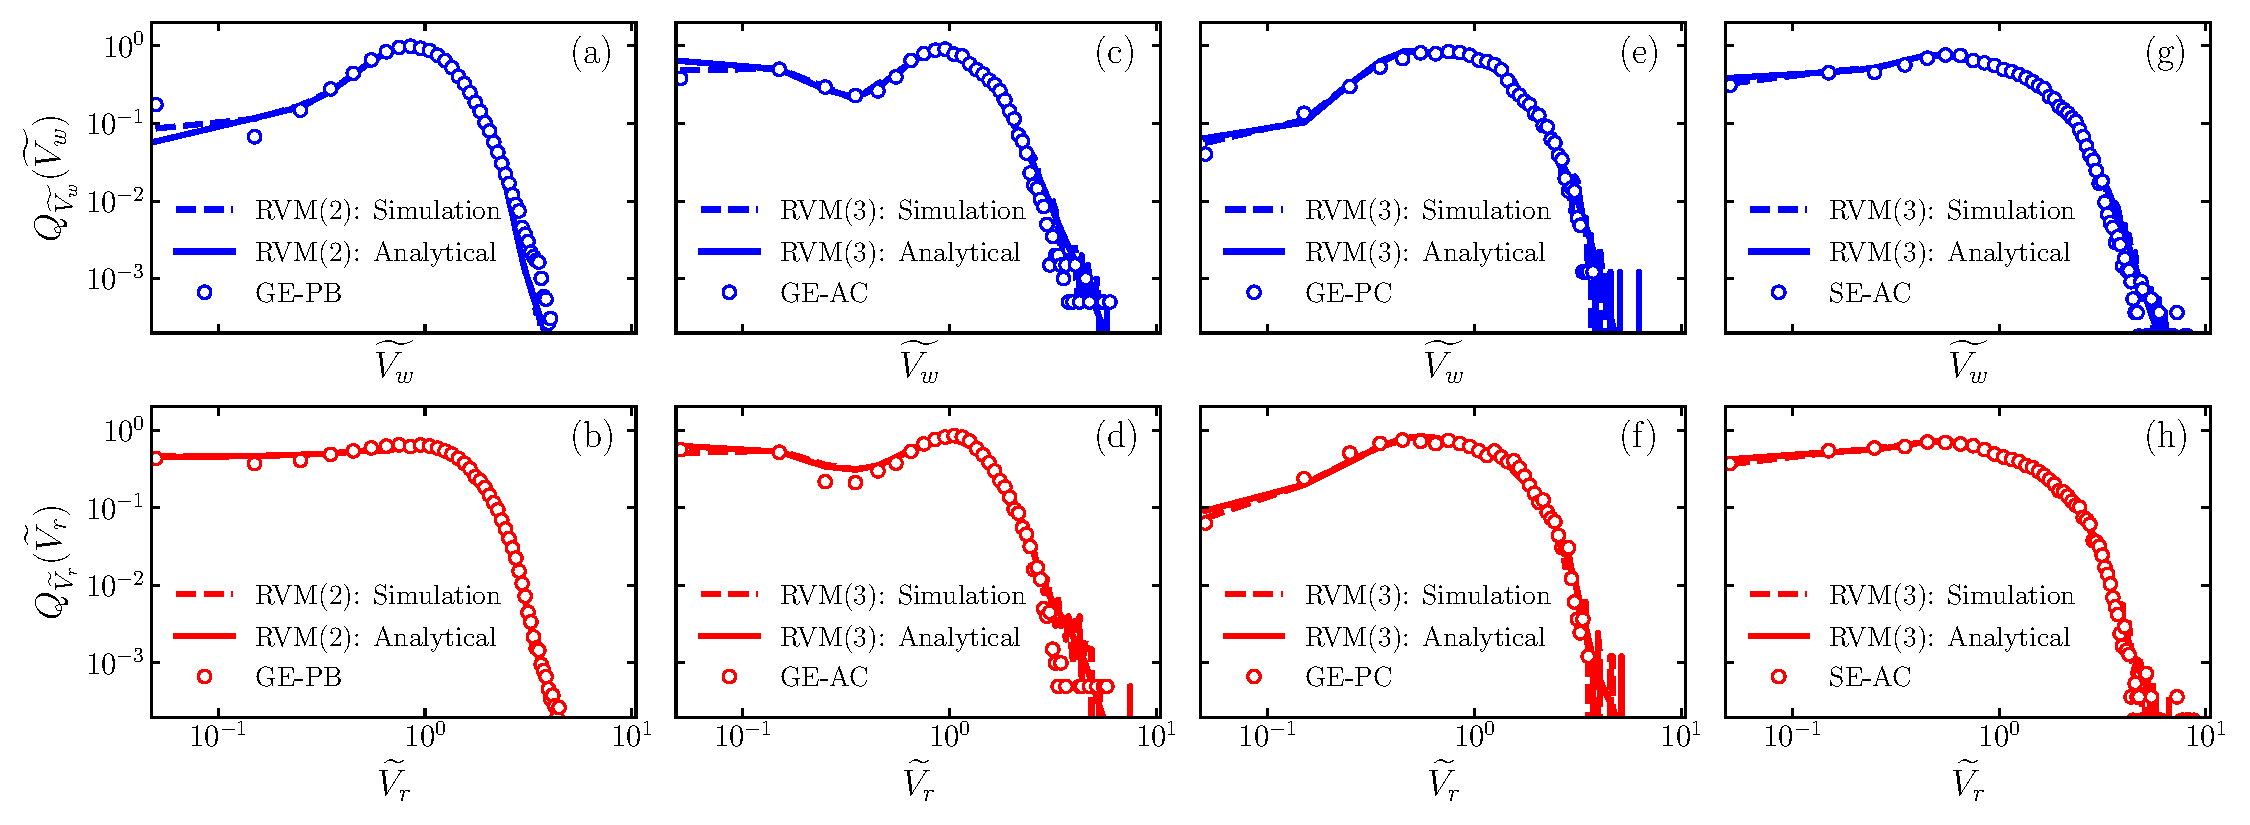
\includegraphics[width=\linewidth]{chapters/chapter6/winner_runnerup_dist_india.pdf}
    \caption{Winner and runner-up vote distributions scaled by their respective means. Panels (a, b), (c, d), and (e, f) depict, respectively, the scaled winner and runner-up vote distribution at the polling booth, assembly constituency, and parliamentary constituency level for Indian general elections. Panels (g, h) correspond to the distributions for the state elections at the assembly constituency level. The analytical predictions (solid lines) are in remarkable agreement with the empirical distributions (open circle). Predictions from RVM simulations (dashed line) closely follow the analytical curves. Note particularly the power-law behavior in the tails ($\widetilde{V} \gg 1$) across all scales, and the distinct profiles at small values ($\widetilde{V} \ll 1$) that vary with the effective number of candidates.}
    \label{fig:winner_runnerup_dist_india}
\end{figure}
\section{Scale Invariance of Margin Distributions in Indian Elections}
Building on our analysis of specific margins $\mu = M/T$ from the previous chapter, we now examine the behavior of the scaled margin distributions $Q_{\widetilde{M}}(\widetilde{M})$ across different electoral scales in India.
\begin{figure}[H]
    \centering
    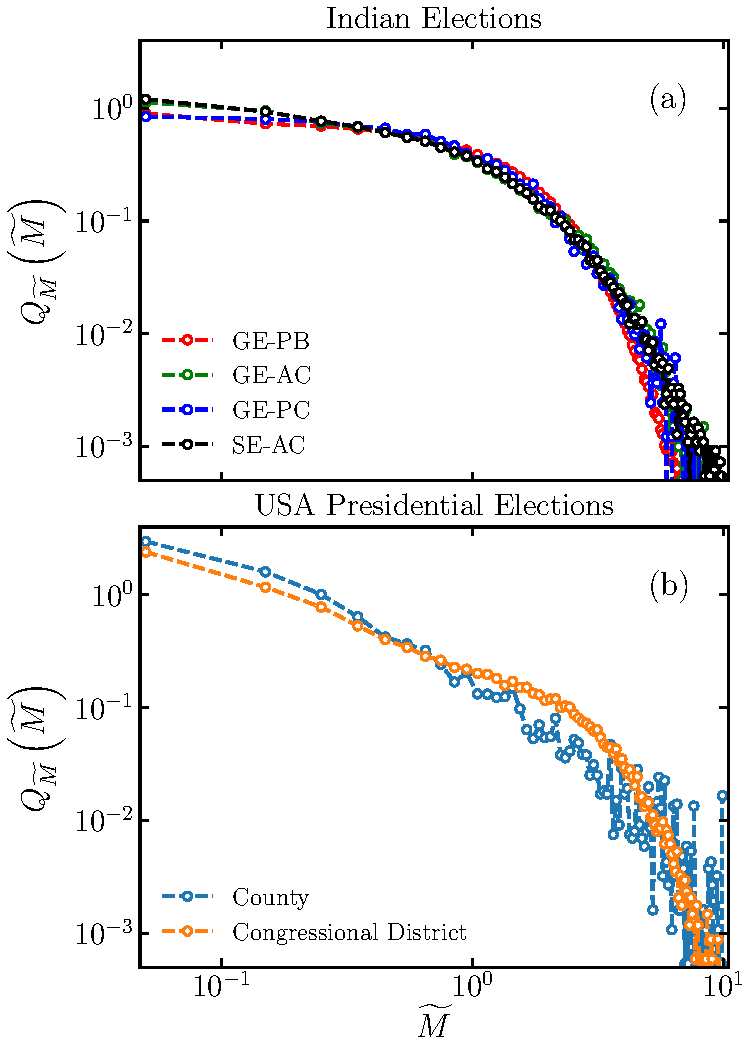
\includegraphics[width=0.8\linewidth]{chapters/chapter6/scaled_margin_dist_India_us.pdf}
    \caption{Margin distributions scaled by their respective means. (a) Data collapse in the scaled margin distributions of Indian elections at four electoral scales. Note how despite the vastly different electoral sizes (from $\sim 10^2$ to $\sim 10^6$ voters), the distributions align remarkably well. (b) In contrast, such collapse is absent in the election data from the USA, where county and district level distributions differ significantly.}
    \label{fig:margin_dist_india_us}
\end{figure}

Remarkably, as demonstrated in Fig.~\ref{fig:margin_dist_india_us} (a), the scaled distributions for the margin for Indian elections at four different scales (GE-PB, GE-AC, GE-PC, and SE-AC) collapse onto a single curve. This data collapse is a direct consequence of the similarity in tail behavior in the corresponding turnout distributions. This appears to be a characteristic feature of Indian elections.

For instance, scaled margin distributions from US elections at the County and Congressional district levels do not exhibit such a collapse (Fig.~\ref{fig:margin_dist_india_us} (b)). This finding highlights a unique characteristic of the Indian electoral system that deserves further investigation.

\section{Conclusion: Turnout Distributions as Electoral Predictors}

In summary, this chapter has demonstrated that voter turnout distributions are not merely indicators of public trust and interest in the electoral process, but they also encode crucial information about several key election statistics. The Random Voting Model, enhanced with the concept of effective number of candidates, provides a powerful framework for predicting various electoral statistics from turnout distributions alone.

Our analysis reveals that voter turnout distributions strongly correlate with winner and runner-up vote distributions, especially at larger electoral scales. This correlation is particularly evident in the remarkable agreement between the analytical predictions from our model and the empirical data. The RVM, when parameterized with the appropriate effective number of candidates ($n^c = 2$ for polling booth level, $n^c = 3$ for constituency levels), accurately predicts the scaled distributions of winner and runner-up votes across different electoral contexts.

Perhaps most striking among our findings is that Indian elections exhibit a unique scale invariance in margin distributions, with scaled margin distributions collapsing onto a single curve across vastly different electoral scales. This phenomenon, not observed in many other democratic systems including the United States, highlights distinctive characteristics of the Indian electoral landscape. Furthermore, the universality of the scaled specific margin distribution is confirmed across multiple electoral scales within India, reinforcing the robustness of our analytical framework.

These findings deepen our understanding of electoral statistics and their relationship with voter turnouts. The predictive power of the RVM framework, using only turnout data and the effective number of candidates as inputs, provides a valuable tool for electoral analysis and could potentially aid in identifying anomalies or irregularities in electoral processes.

As we move to the next chapter, we will explore the practical applications of these insights, focusing on designing interventions and developing methods to flag electoral malpractice based on deviations from the expected statistical patterns.
